\documentclass[landscape,final,a0paper,fontscale=0.285]{baposter}

\usepackage{calc}
\usepackage{graphicx}
\usepackage{amsmath}
\usepackage{amssymb}
\usepackage{relsize}
\usepackage{multirow}
\usepackage{rotating}
\usepackage{bm}
\usepackage{url}
\usepackage{graphicx}
\usepackage{multicol}
\usepackage{palatino}

\newcommand{\captionfont}{\footnotesize}
\usetikzlibrary{calc}
\newcommand{\SET}[1]  {\ensuremath{\mathcal{#1}}}
\newcommand{\MAT}[1]  {\ensuremath{\boldsymbol{#1}}}
\newcommand{\VEC}[1]  {\ensuremath{\boldsymbol{#1}}}
\newcommand{\Video}{\SET{V}}
\newcommand{\video}{\VEC{f}}
\newcommand{\track}{x}
\newcommand{\Track}{\SET T}
\newcommand{\LMs}{\SET L}
\newcommand{\lm}{l}
\newcommand{\PosE}{\SET P}
\newcommand{\posE}{\VEC p}
\newcommand{\negE}{\VEC n}
\newcommand{\NegE}{\SET N}
\newcommand{\Occluded}{\SET O}
\newcommand{\occluded}{o}

\graphicspath{{images/}{../images/}}

%%%%%%%%%%%%%%%%%%%%%%%%%%%%%%%%%%%%%%%%%%%%%%%%%%%%%%%%%%%%%%%%%%%%%%%%%%%%%%%%
%%%% Some math symbols used in the text
%%%%%%%%%%%%%%%%%%%%%%%%%%%%%%%%%%%%%%%%%%%%%%%%%%%%%%%%%%%%%%%%%%%%%%%%%%%%%%%%

%%%%%%%%%%%%%%%%%%%%%%%%%%%%%%%%%%%%%%%%%%%%%%%%%%%%%%%%%%%%%%%%%%%%%%%%%%%%%%%%
% Multicol Settings
%%%%%%%%%%%%%%%%%%%%%%%%%%%%%%%%%%%%%%%%%%%%%%%%%%%%%%%%%%%%%%%%%%%%%%%%%%%%%%%%
\setlength{\columnsep}{1.5em}
\setlength{\columnseprule}{0mm}

%%%%%%%%%%%%%%%%%%%%%%%%%%%%%%%%%%%%%%%%%%%%%%%%%%%%%%%%%%%%%%%%%%%%%%%%%%%%%%%%
% Save space in lists. Use this after the opening of the list
%%%%%%%%%%%%%%%%%%%%%%%%%%%%%%%%%%%%%%%%%%%%%%%%%%%%%%%%%%%%%%%%%%%%%%%%%%%%%%%%
\newcommand{\compresslist}{%
\setlength{\itemsep}{1pt}%
\setlength{\parskip}{0pt}%
\setlength{\parsep}{0pt}%
}

%%%%%%%%%%%%%%%%%%%%%%%%%%%%%%%%%%%%%%%%%%%%%%%%%%%%%%%%%%%%%%%%%%%%%%%%%%%%%%
%%% Begin of Document
%%%%%%%%%%%%%%%%%%%%%%%%%%%%%%%%%%%%%%%%%%%%%%%%%%%%%%%%%%%%%%%%%%%%%%%%%%%%%%

\begin{document}

%%%%%%%%%%%%%%%%%%%%%%%%%%%%%%%%%%%%%%%%%%%%%%%%%%%%%%%%%%%%%%%%%%%%%%%%%%%%%%
%%% Here starts the poster
%%%---------------------------------------------------------------------------
%%% Format it to your taste with the options
%%%%%%%%%%%%%%%%%%%%%%%%%%%%%%%%%%%%%%%%%%%%%%%%%%%%%%%%%%%%%%%%%%%%%%%%%%%%%%
% Define some colors

%\definecolor{lightblue}{cmyk}{0.83,0.24,0,0.12}
\definecolor{lightblue}{rgb}{0.145,0.6666,1}

\hyphenation{resolution occlusions}
%%
\begin{poster}%
  % Poster Options
  {
    % Column spacing
    colspacing=1em,
    % Color style
    bgColorOne=white,
    bgColorTwo=white,
    borderColor=lightblue,
    headerColorOne=black,
    headerColorTwo=lightblue,
    headerFontColor=white,
    boxColorOne=white,
    boxColorTwo=lightblue,
    % Format of textbox
    textborder=roundedleft,
    background=none,
    % Format of text header
    eyecatcher=true,
    headerborder=open,
    headerheight=0.1\textheight,
    headershape=roundedright,
    headershade=shadelr,
    headerfont=\Large\bf\textsc, %Sans Serif
    textfont={\setlength{\parindent}{1.5em}},
    boxshade=plain,
    background=plain,
    linewidth=2pt
  }
  % Eye Catcher
  {
\includegraphics[height=7em]{images/workflow.png}}
  % Title
  {\bf\textsc{Visual Work-Flows for OpenShift}\vspace{0.5em}}
  % Authors
  {\small{\textsc{Sanchit Aggarwal~~~~Sandeep Panem~~~~Subho Banerjee~~~~Vijayendra Grampurohit}}}
  % University logo
  {
\includegraphics[height=6em]{images/siel.png}
\includegraphics[height=6em]{images/cloud.png}}

%%%%%%%%%%%%%%%%%%%%%%%%%%%%%%%%%%%%%%%%%%%%%%%%%%%%%%%%%%%%%%%%%%%%%%%%%%%%%%
  \headerbox{Problem}{name=problem,column=0,row=0}{
%%%%%%%%%%%%%%%%%%%%%%%%%%%%%%%%%%%%%%%%%%%%%%%%%%%%%%%%%%%%%%%%%%%%%%%%%%%%%%
  \noindent Identify enterprise work-flows for deploying applications to Openshift and build a client which provides an interface to the Broker-API for simple deployments as well as more complicated work-flows using --
  \vspace{-0.2em}
   \begin{enumerate}\compresslist
      \item Keystone authentication
      \item Openshift REST API
      \item Abstract interface to create your own work-flows
   \end{enumerate}
   \vspace{0.2em}
 }

%%%%%%%%%%%%%%%%%%%%%%%%%%%%%%%%%%%%%%%%%%%%%%%%%%%%%%%%%%%%%%%%%%%%%%%%%%%%%%
  \headerbox{Contributions}{name=contribution,column=1,row=0,bottomaligned=problem}{
%%%%%%%%%%%%%%%%%%%%%%%%%%%%%%%%%%%%%%%%%%%%%%%%%%%%%%%%%%%%%%%%%%%%%%%%%%%%%%
  \noindent We designed and implemented a system which can take as an input, an enterprise workflow for Openshift and then deploys it to the cloud. Some salient features of our project are --
  \begin{enumerate}\compresslist
    \item \texttt{HTML5} based drag and drop interface for building work-flows.
    \item Ability to deploy to all Openshift distributions
    \item Extensible
  \end{enumerate}
  \vspace{0.5em}
}

%%%%%%%%%%%%%%%%%%%%%%%%%%%%%%%%%%%%%%%%%%%%%%%%%%%%%%%%%%%%%%%%%%%%%%%%%%%%%%
  \headerbox{Architecture}{name=arch,column=2,span=2,row=0}{
%%%%%%%%%%%%%%%%%%%%%%%%%%%%%%%%%%%%%%%%%%%%%%%%%%%%%%%%%%%%%%%%%%%%%%%%%%%%%%
  \noindent\begin{tabular}{cc}
    \begin{minipage}{0.5\linewidth}
      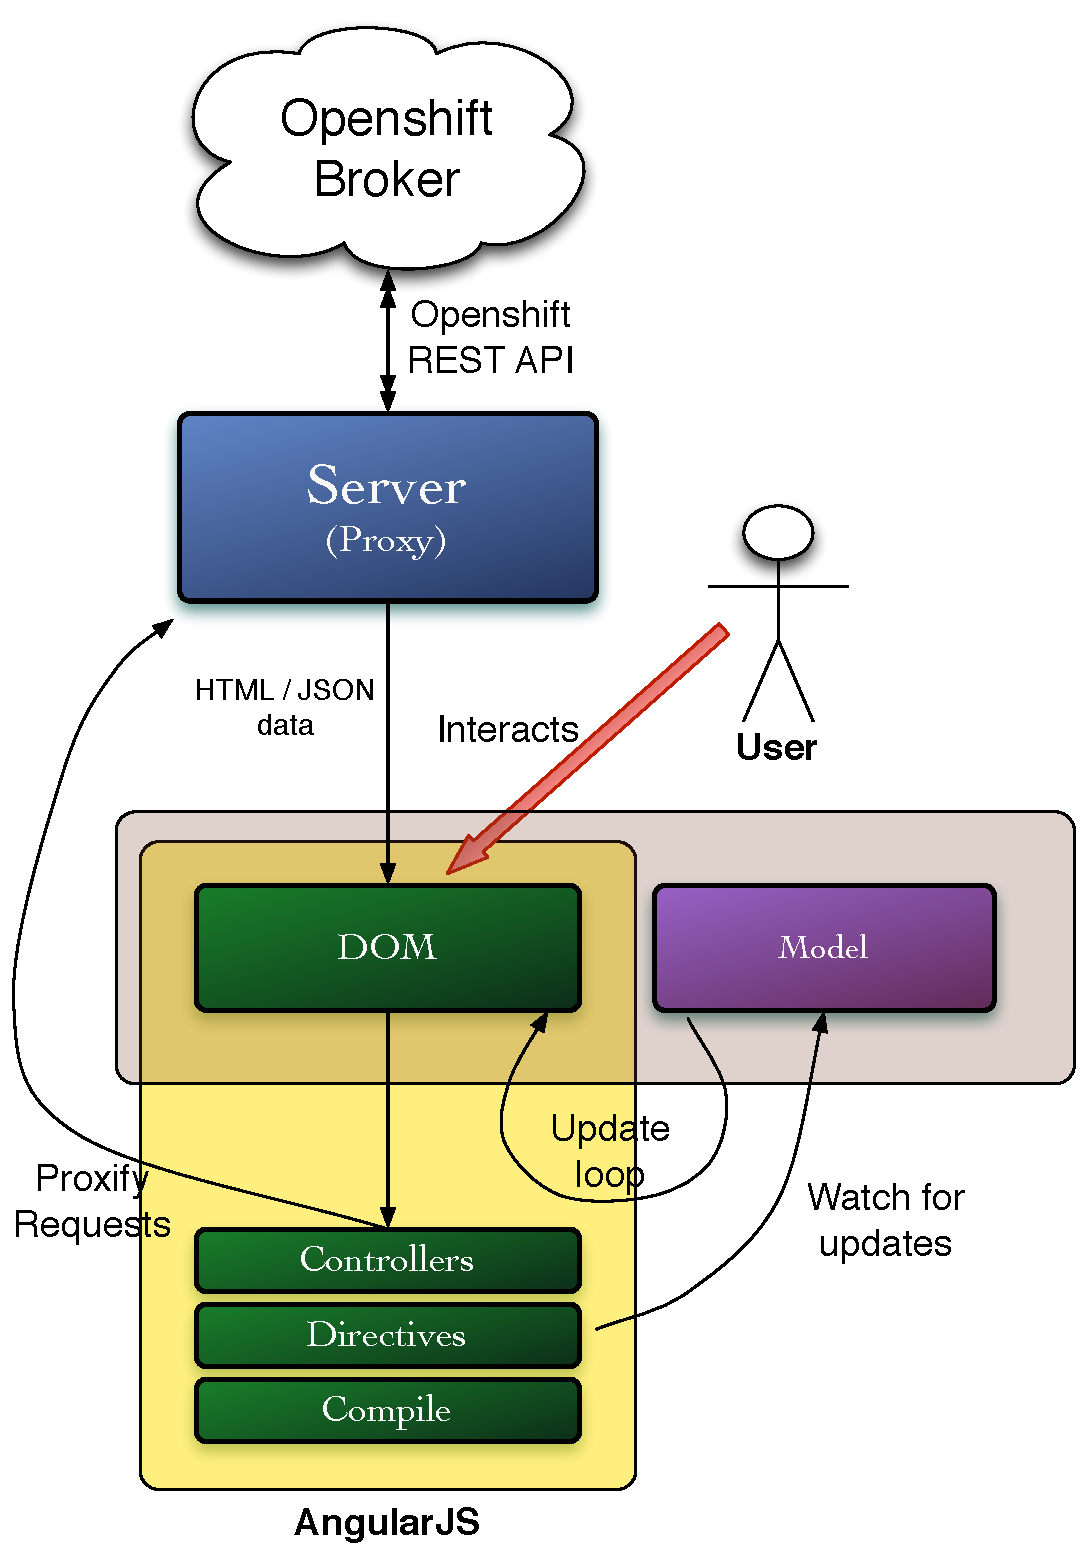
\includegraphics[width=0.85\linewidth]{images/arch.pdf}
    \end{minipage}&
    \begin{minipage}{0.5\linewidth}
      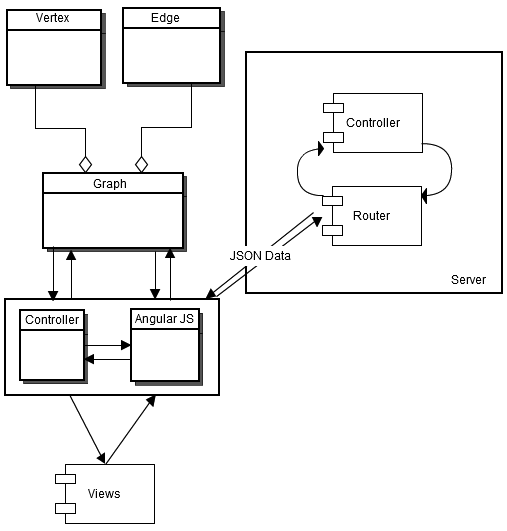
\includegraphics[width=0.9\linewidth]{images/class.png}
    \end{minipage}
  \end{tabular}\\[1em]
  \vspace{0.3em}
}

%%%%%%%%%%%%%%%%%%%%%%%%%%%%%%%%%%%%%%%%%%%%%%%%%%%%%%%%%%%%%%%%%%%%%%%%%%%%%%
  \headerbox{Screenshots}{name=product,below=arch,column=2,span=2}{
%%%%%%%%%%%%%%%%%%%%%%%%%%%%%%%%%%%%%%%%%%%%%%%%%%%%%%%%%%%%%%%%%%%%%%%%%%%%%%
  \begin{center}
    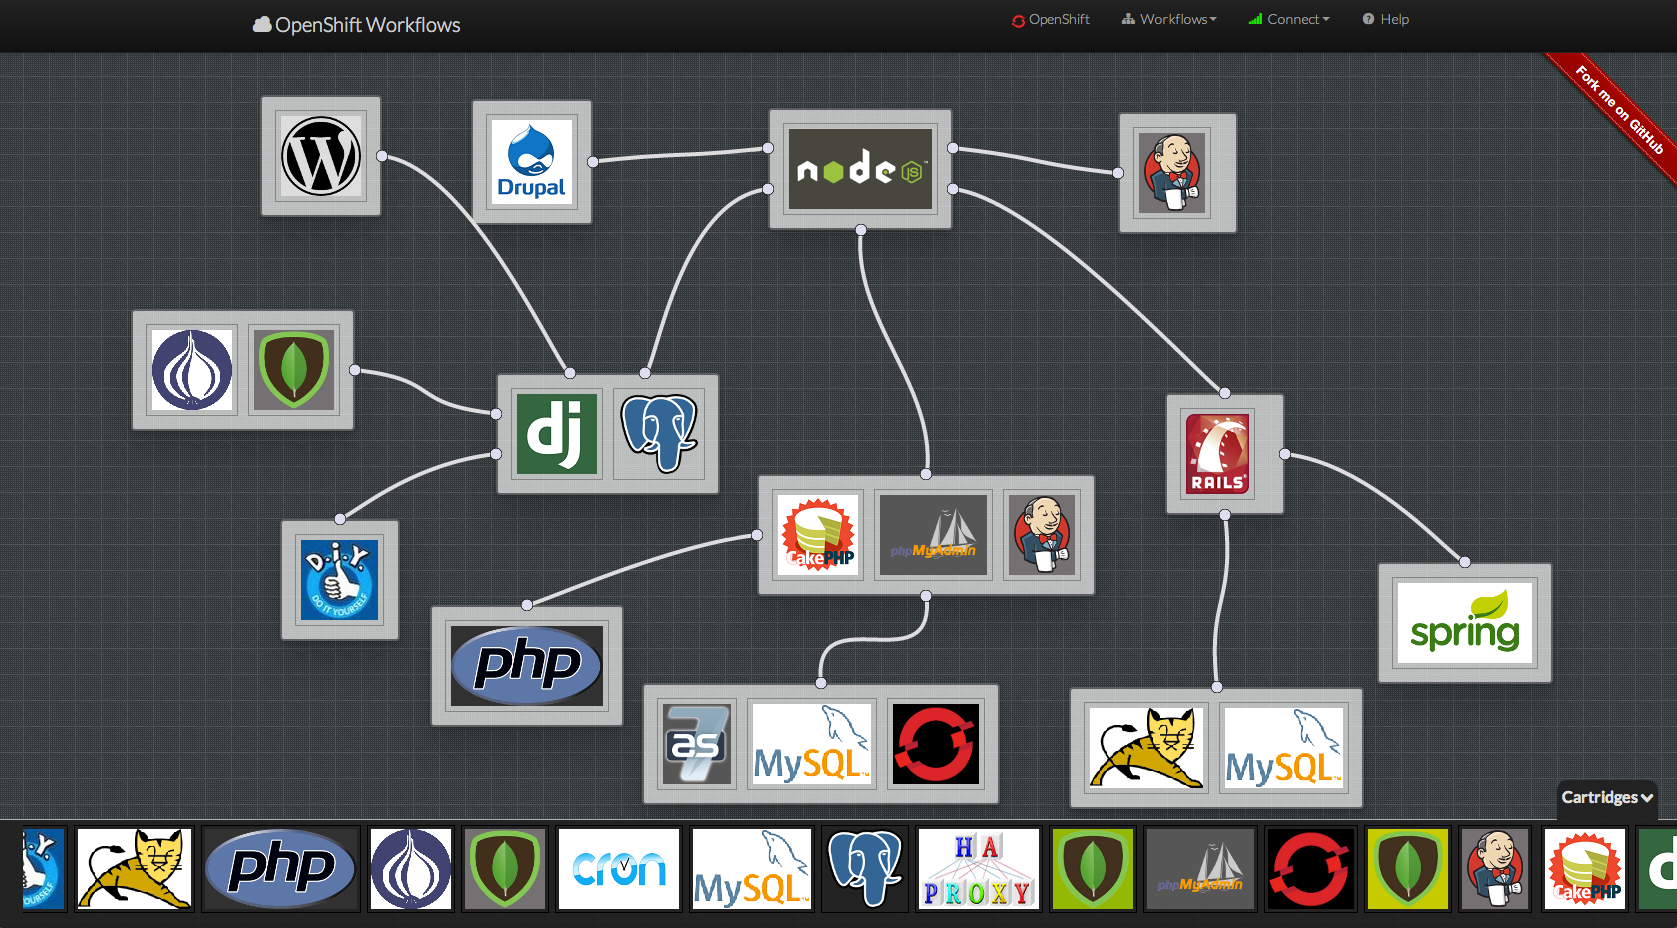
\includegraphics[width=22em]{images/screenshot_1.png}
    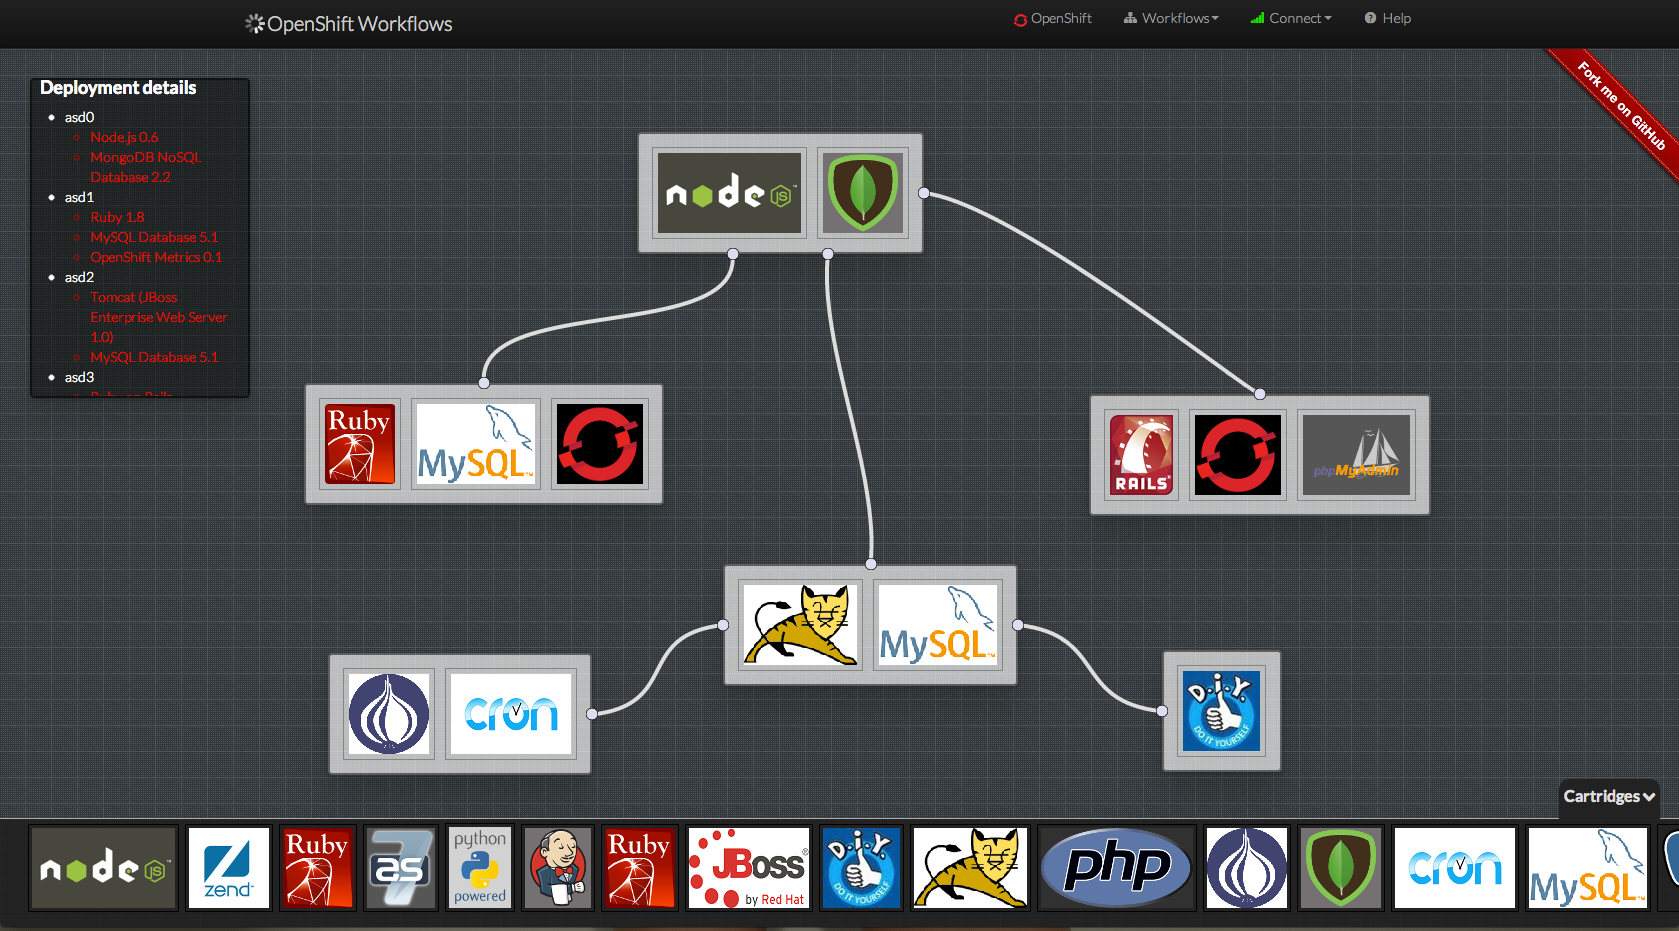
\includegraphics[width=22em]{images/screenshot_2.png}
  \end{center}
}

%%%%%%%%%%%%%%%%%%%%%%%%%%%%%%%%%%%%%%%%%%%%%%%%%%%%%%%%%%%%%%%%%%%%%%%%%%%%%%
  \headerbox{User Interactions}{name=interactions,below=problem,column=0,span=2,bottomaligned=product}{
%%%%%%%%%%%%%%%%%%%%%%%%%%%%%%%%%%%%%%%%%%%%%%%%%%%%%%%%%%%%%%%%%%%%%%%%%%%%%%
  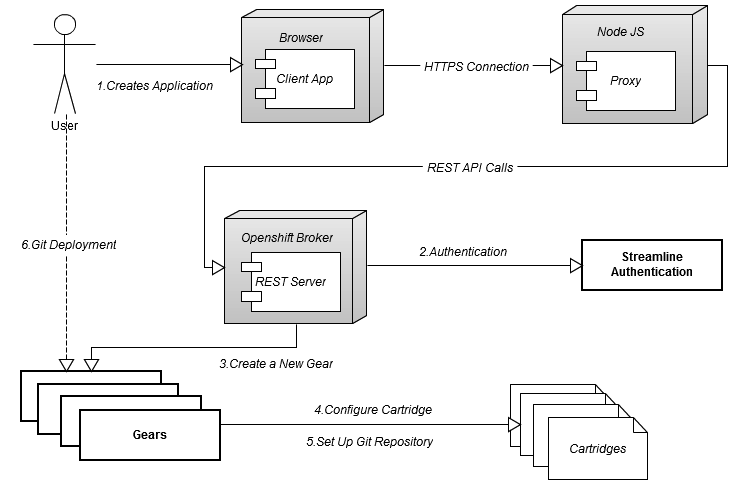
\includegraphics[width=0.9\linewidth]{images/interactions.png}
}

%%%%%%%%%%%%%%%%%%%%%%%%%%%%%%%%%%%%%%%%%%%%%%%%%%%%%%%%%%%%%%%%%%%%%%%%%%%%%%
  \headerbox{Technologies Used}{name=tech,column=0,below=interactions}{
%%%%%%%%%%%%%%%%%%%%%%%%%%%%%%%%%%%%%%%%%%%%%%%%%%%%%%%%%%%%%%%%%%%%%%%%%%%%%%
  
\includegraphics[width=0.4\linewidth]{images/nodejs.png}
  
\includegraphics[width=0.1\linewidth]{images/html5.png}
  
\includegraphics[width=0.4\linewidth]{images/angularjs.png}\\[0.7em]
  
\includegraphics[width=0.4\linewidth]{images/jquery.png}
  
\includegraphics[width=0.1\linewidth]{images/bootstrap.png}
  
\includegraphics[width=0.4\linewidth]{images/jqueryui.png}
}

%%%%%%%%%%%%%%%%%%%%%%%%%%%%%%%%%%%%%%%%%%%%%%%%%%%%%%%%%%%%%%%%%%%%%%%%%%%%%%
  \headerbox{Future Work}{name=future,column=1,span=2,aligned=references,below=product,bottomaligned=tech}{
%%%%%%%%%%%%%%%%%%%%%%%%%%%%%%%%%%%%%%%%%%%%%%%%%%%%%%%%%%%%%%%%%%%%%%%%%%%%%%
  \begin{multicols}{2}
    We would like to extend the application to managing deployed apps as well. Particularly, setting auto-scale parameters and controlling the life-cycle.

    We would also like to add a mechanism by which the user can directly deploy his code using our portal rather than having to synchronize \texttt{Git} repositories manually.
  \end{multicols}
}

%%%%%%%%%%%%%%%%%%%%%%%%%%%%%%%%%%%%%%%%%%%%%%%%%%%%%%%%%%%%%%%%%%%%%%%%%%%%%%
  \headerbox{Source Code}{name=references,column=3,aligned=tech,below=product,bottomaligned=tech}{
%%%%%%%%%%%%%%%%%%%%%%%%%%%%%%%%%%%%%%%%%%%%%%%%%%%%%%%%%%%%%%%%%%%%%%%%%%%%%%
  \noindent\begin{tabular}{cc}
    \begin{minipage}{0.8\linewidth}
      The source code for the back and front end is available available at\\ \url{https://github.com/subszero/openshift-workflows}
    \end{minipage}&
    \begin{minipage}{0.2\linewidth}
      
\includegraphics[width=0.7\linewidth]{images/github.png}
    \end{minipage}
  \end{tabular}\\[1em]
  \vspace{0.3em}
}

\end{poster}

\end{document}
